\begin{figure}
\centering

\def\picScale{0.08}    % define variable for scaling all pictures evenly
\def\colWidth{0.5\linewidth}

\begin{tikzpicture}
\matrix [row sep=0.25cm, column sep=0cm, style={align=center}] (my matrix) at (0,0) %(2,1)
{
\node[style={anchor=center}] (FREEhand) {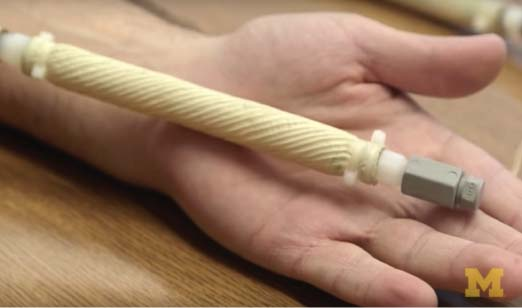
\includegraphics[width=0.85\linewidth]{figures/FREEhand.jpg}}; %\fill[blue] (0,0) circle (2pt);
\\
\node[style={anchor=center}] (rigid_v_soft) {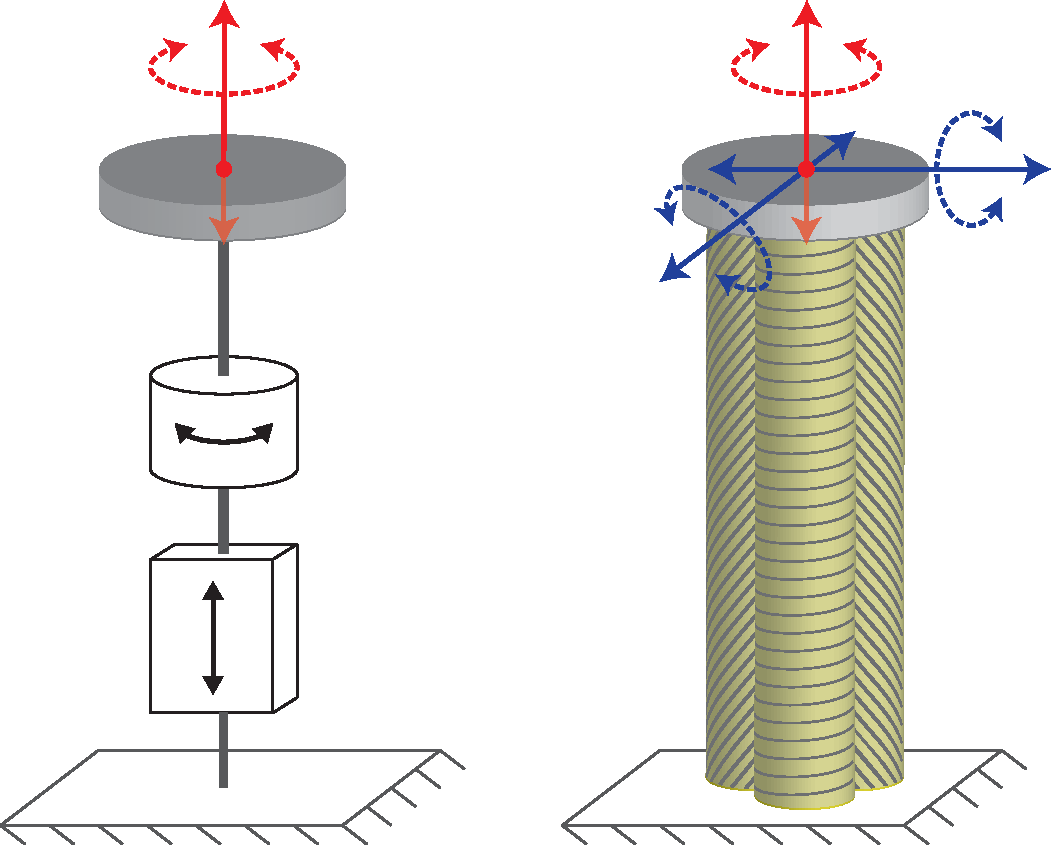
\includegraphics[width=0.75\linewidth]{figures/FREE_vs_rigid-v8.pdf}}; %\fill[blue] (0,0) circle (2pt);
\\
};
\node[above] (FREEhand) at ($ (FREEhand.south west)  !0.05! (FREEhand.south east) + (0, 0.1)$) {(a)};
\node[below] (a) at ($ (rigid_v_soft.south west) !0.20! (rigid_v_soft.south east) $) {(b)};
\node[below] (b) at ($ (rigid_v_soft.south west) !0.75! (rigid_v_soft.south east) $) {(c)};
\end{tikzpicture}


% \begin{tikzpicture} %[every node/.style={draw=black}]
% % \draw[help lines] (0,0) grid (4,2);
% \matrix [row sep=0cm, column sep=0cm, style={align=center}] (my matrix) at (0,0) %(2,1)
% {
% \node[style={anchor=center}] {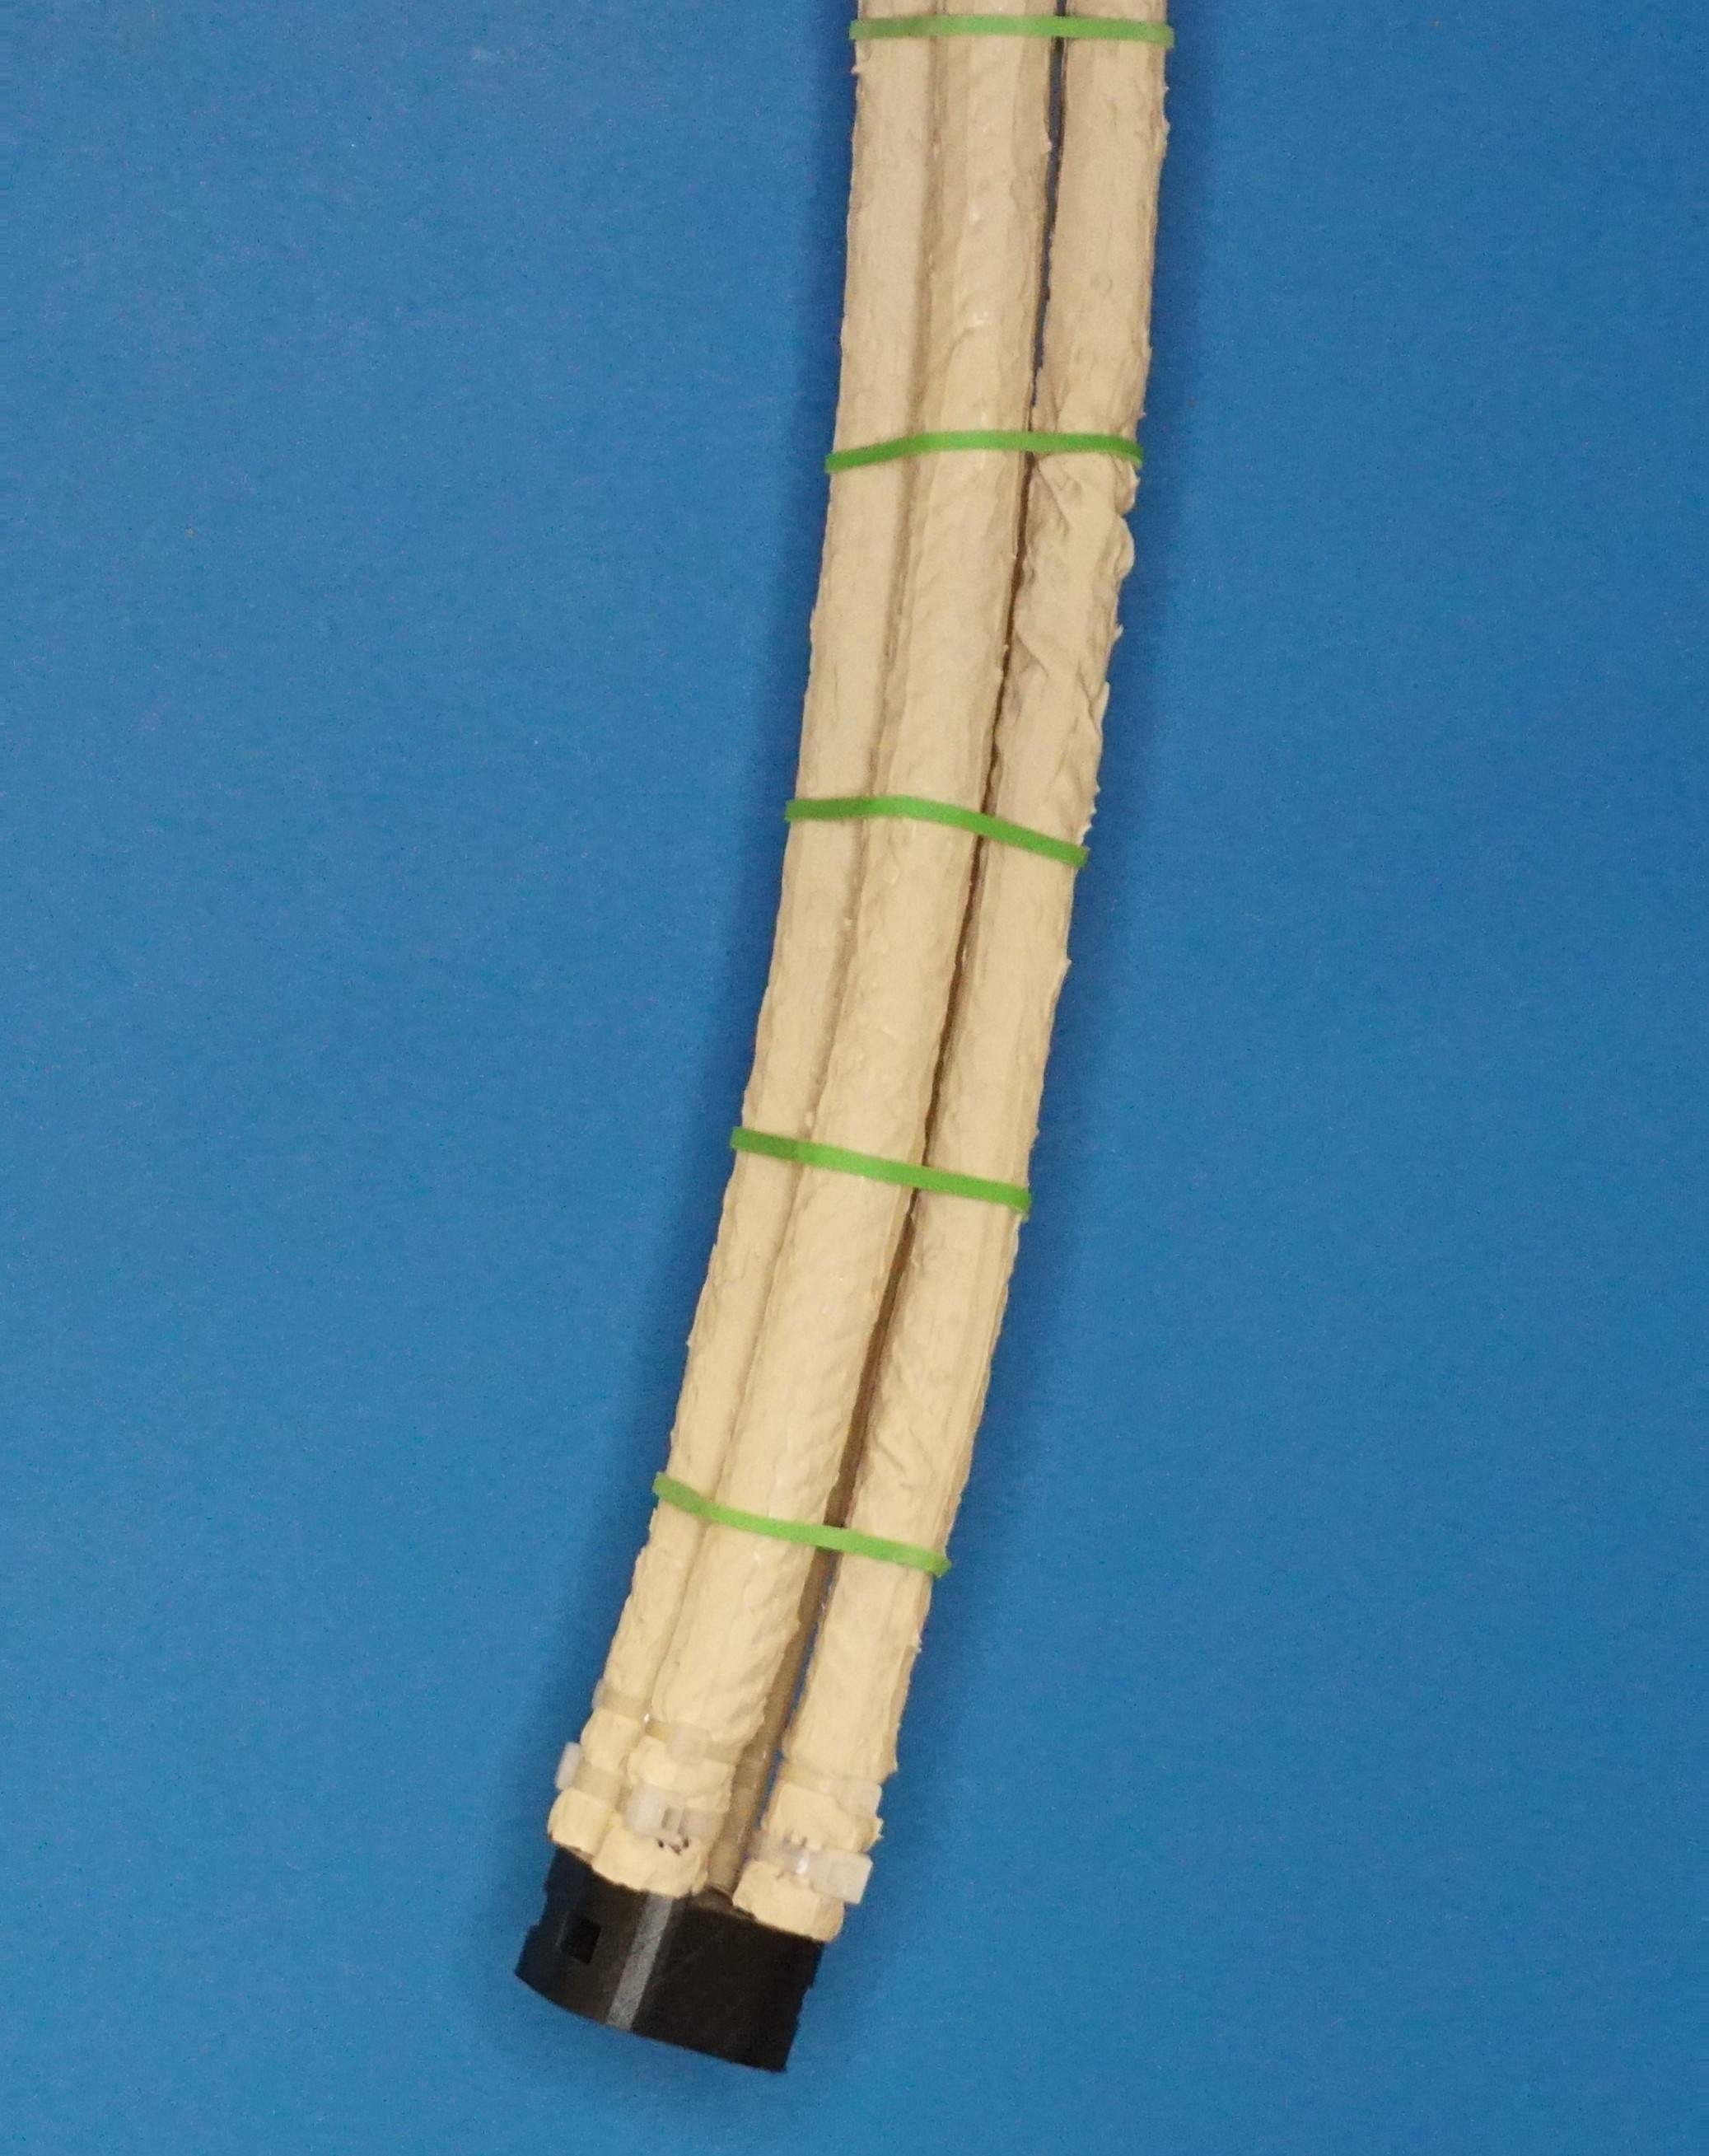
\includegraphics[width=\colWidth]{figures/photos/labFREEs3.jpg}}; %\fill[blue] (0,0) circle (2pt)
% &
% \node[style={anchor=center}] {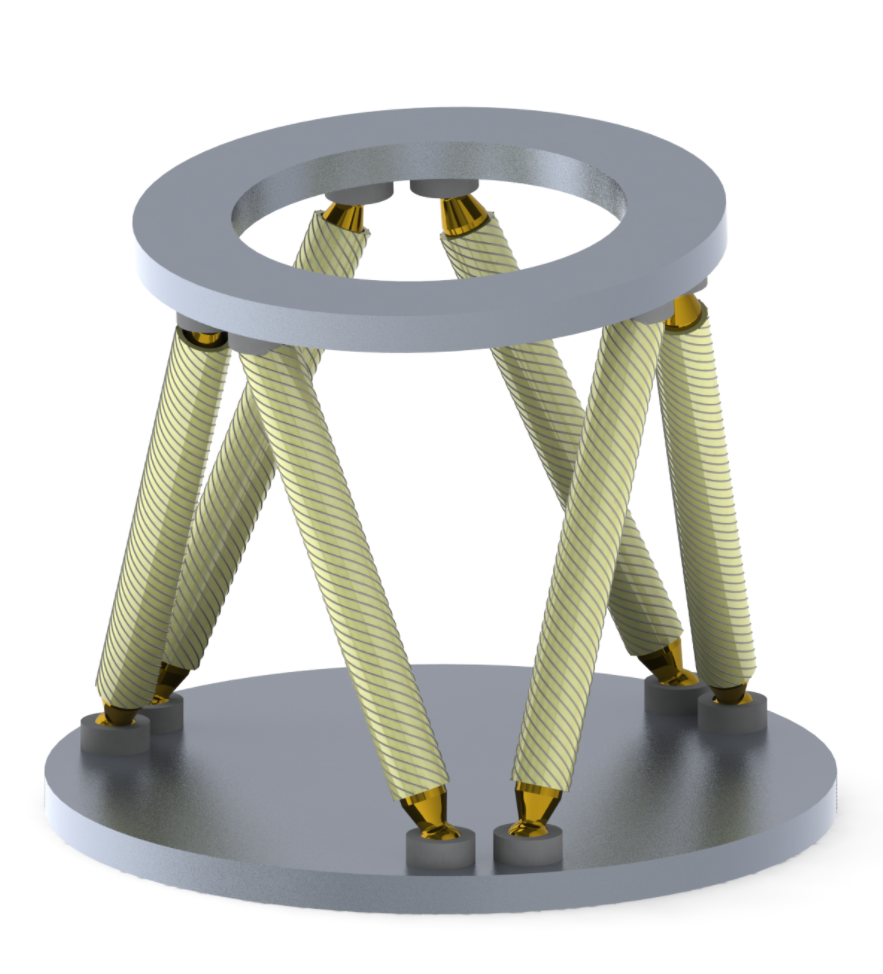
\includegraphics[width=\colWidth, height=160pt]{figures/stewartRender.png}}; %\fill[blue] (0,0) circle (2pt);
% \\
% };

% %\node[style={anchor=center}] at (0,-5) (FREEstate) {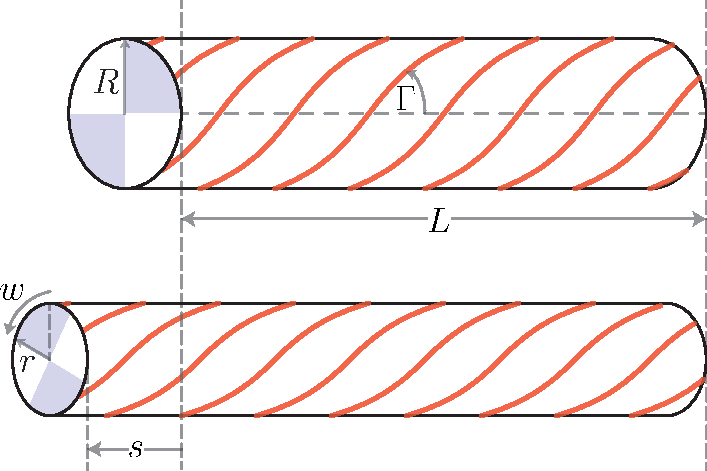
\includegraphics[width=0.7\linewidth]{figures/FREEstate_noLabels2.pdf}};

% \end{tikzpicture}

\caption{\revcomment{2.3}{(a) A fiber-reinforced elastomerc enclosure (FREE) is a soft fluid-driven actuator composed of an elastomer tube with fibers wound around it to impose specific deformations under an increase in volume, such as extension and torsion. (b) A linear actuator and motor combined in \emph{series} has the ability to generate 2 dimensional forces at the end effector (shown in red), but is constrained to motions only in the directions of these forces. (b) Three FREEs combined in \emph{parallel} can generate the same 2 dimensional forces at the end effector (shown in red), without imposing kinematic constraints that prohibit motion in other directions (shown in blue).}}

% \caption{A fiber-reinforced elastomeric enclosure (FREE) (top) is a soft fluid-driven actuator composed of an elastomer tube with fibers wound around it to impose deformation in specific directions upon pressurization, such as extension and torsion. \revcomment{2.3}{In this paper we explore the potential of combining multiple FREEs in parallel to generate fully controllable multi-dimensional spacial forces}, such as in a parallel arrangement around a flexible spine element (bottom-left), or a Stewart Platform arrangement (bottom-right).}

\label{fig:overview}
\end{figure}
